\section{Physical Architectural View}

As previously mentioned, there are many layers of abstraction in the program before any function call actually reaches the hardware level of the sensors. In this section, we will describe these layers, going from the high-level programming of the model, e.g. the architecture described in Figure \ref{fig:softwareArchitecture}, down to the hardware specifics of the sensors themselves. 

The intent is, of course, that these software abstractions will not affect our model implementation, aside from the fact that we have to include some libraries to facilitate sensor communication (for instance \code{ecrobot\_interface.h} and similar). Still, it is important to understand how the software actually communicates with the hardware. 

See Figure \ref{fig:abstractionLayers} for the system architecture and how data flows through its layers of abstraction. The diagram is loosely based on the OSI layer diagram that shows abstraction levels. One key change is that the arrows represent the flow of data; arrowhead pointing towards the receiver. 

\begin{figure}[H]
    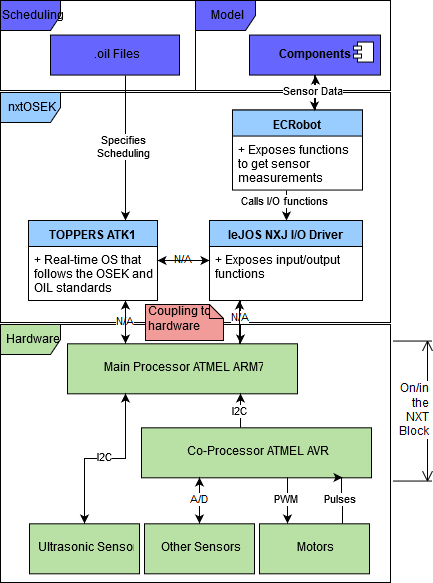
\includegraphics[width=\textwidth]{Images/Design/abstractionLayerDiagram.png}
    \caption{Layer diagram of the system architecture of the product, going from high-level programming down to low-level hardware specifics.}
    \label{fig:abstractionLayers}
\end{figure}

%\todo[inline]{From supervisor: These arrows mean different things than other arrows inside the box, so they must be drawn somehow differently.}

The dark blue coloured area contains all the software that we will write, the light blue area contains software supplied by the nxtOSEK operating system and the green area contains the hardware on the physical bus. 

The note "Coupling to hardware" is written because those are implementation details within nxtOSEK \todo{From supervisor: Just treat it as a different abstraction layer. It is not realy an API, nor protocol, but something that "runs on top". Response: I don't know what to change to achieve this. Seems good to me?}. In the hardware frame, the edges signify communication protocols such as PWM (pulse width modulation, which has been described in section \ref{analysisMotors}). 
